\subsection{Baumstruktur}
\label{subsec:tree}
Die Baumstruktur ist dafür gedacht, Elemente zu repräsentieren, die wiederum Unterelemente
enthalten können. Ein klassisches Beispiel ist dabei ein \emph{Filesystem}. Es existieren in
einem \emph{Filesystem} sowohl \emph{Ordner} als auch \emph{Dateien}. Ein \emph{Odner} kann
sowohl mehrere \emph{Dateien} als auch weitere \emph{Ordner} in sich tragen. In den weiteren
\emph{Ordnern} können sich wieder Elemente befinden.

In diesem Szenario wurden jeweils \emph{NxM} Bäume erzeugt. Dabei steht \emph{N} für die Anzahl
der übergeordneten Elementen und \emph{M} für die Anzahl der untergeordneten Elementen. Die
Ergebnisse der Messungen resultierten in das folgende Diagram:

\begin{figure}[h]
    \centering
    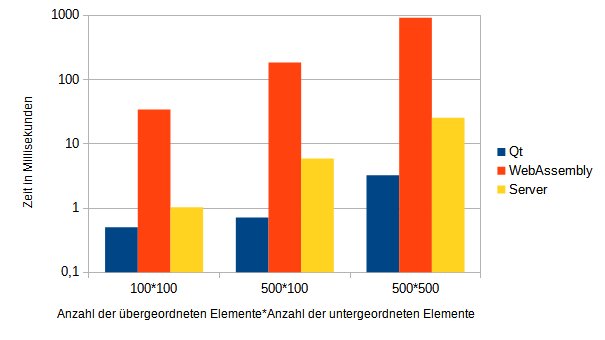
\includegraphics[width=\textwidth, center]{Analyse/Tree}
    \caption[Ergebnisse der Messungen von der Erzeugung einer Baumstruktur in
    Millisekunden]{Ergebnisse
    der Messungen von der Erzeugung einer Baumstruktur in Millisekunden}
    \label{img:table}
\end{figure}

In diesem Diagram, ist zu erkennen, das hier die Server-Architektur performanter als die
WebAssembly-Architektur ist. Dies könnte dadurch erklärt werden, da hier mit wesentlich weniger
Elementen gearbeitet wurde als in der Sektion \emph{\nameref{subsec:table}}. Dadurch müssen nicht
so viele Elemente vom Server zum Browser übertragen werden.